\subsection{StyleCLIP}
\begin{frame}[allowframebreaks]{StyleCLIP}
    \textbf{StyleCLIP} is a method that combines the power of CLIP (Contrastive Language-Image Pretraining) with StyleGAN to generate images based on text prompts, allowing for fine-grained control over image attributes.

    \begin{itemize}
        \item \textbf{CLIP Embeddings:} Uses CLIP to encode text prompts into embeddings that capture semantic information.
        \item \textbf{StyleGAN Manipulation:} Applies these embeddings to manipulate the latent space of StyleGAN, enabling the generation of images that match the desired attributes described in the text.
        \item \textbf{Applications:} Useful for tasks like image editing, attribute manipulation, and creative content generation.
        \item \textbf{Benefits:} Provides a powerful way to generate diverse images based on textual descriptions.
        \item \textbf{Costs:} Requires careful tuning of the StyleGAN latent space and may produce artifacts if not managed properly.
    \end{itemize}
\framebreak
    \begin{figure}
        \centering
        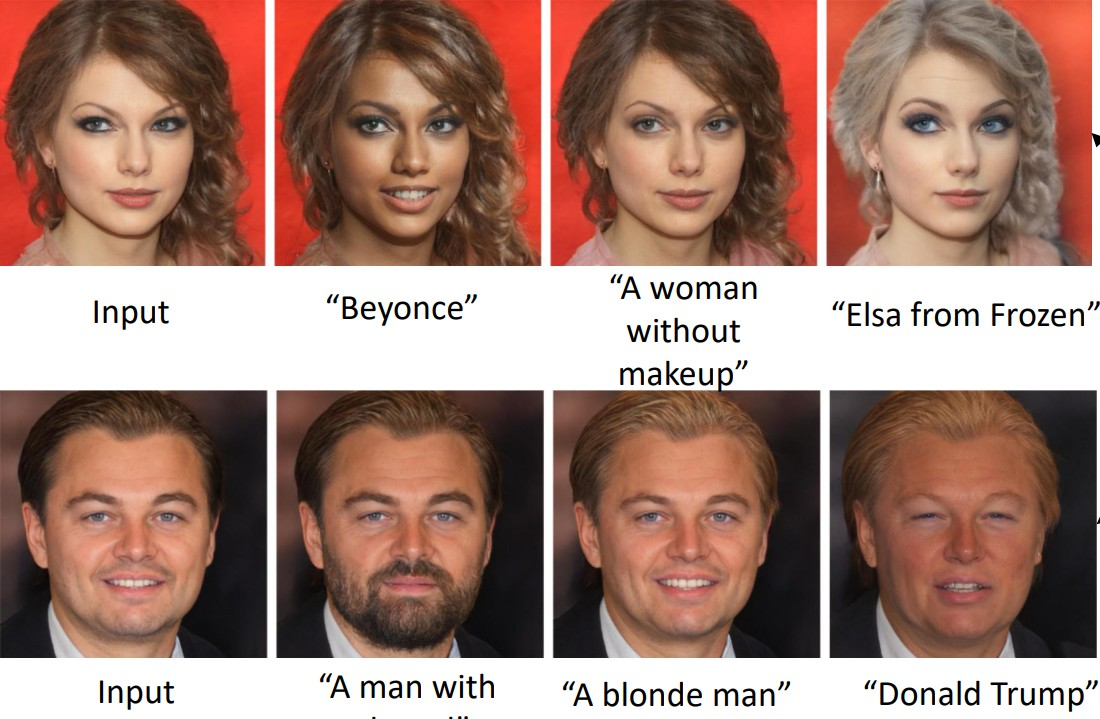
\includegraphics[width=1\textwidth,height=0.9\textheight,keepaspectratio]{images/video/slide_65_1_img.jpg}
    \end{figure}
\framebreak
    \begin{figure}
        \centering
        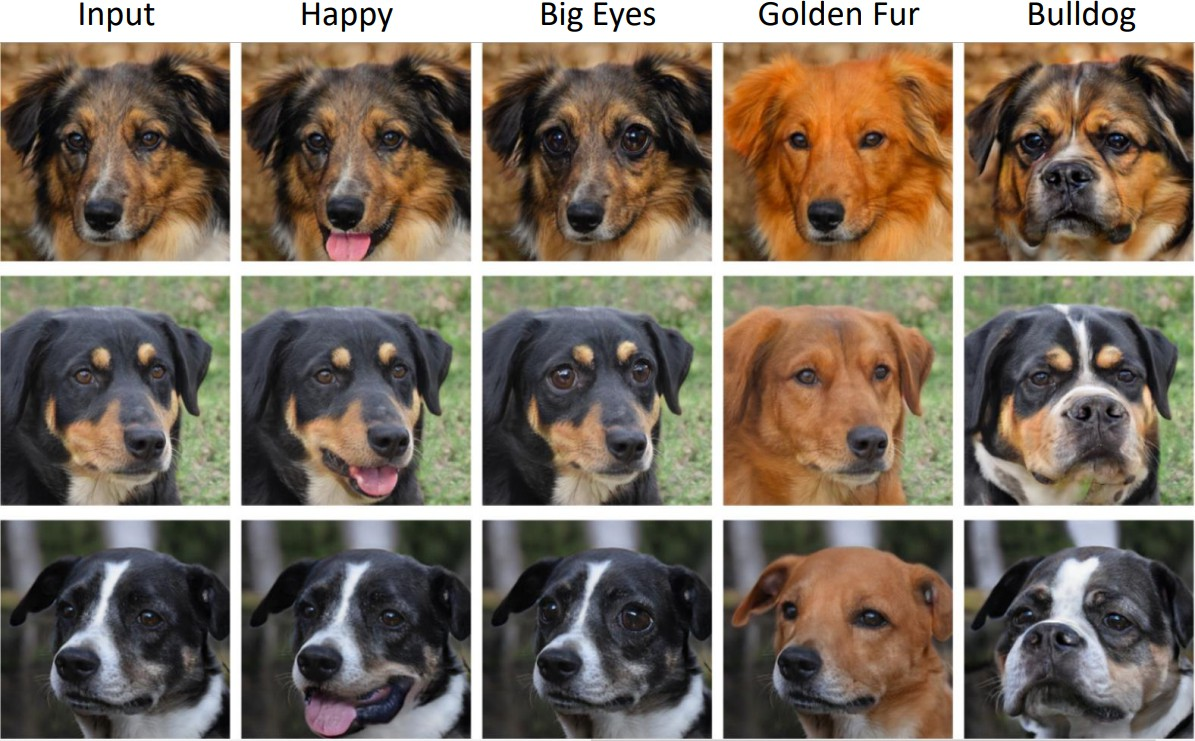
\includegraphics[width=1\textwidth,height=0.9\textheight,keepaspectratio]{images/video/slide_66_1_img.jpg}
    \end{figure}

\framebreak
    \begin{figure}
        \centering
        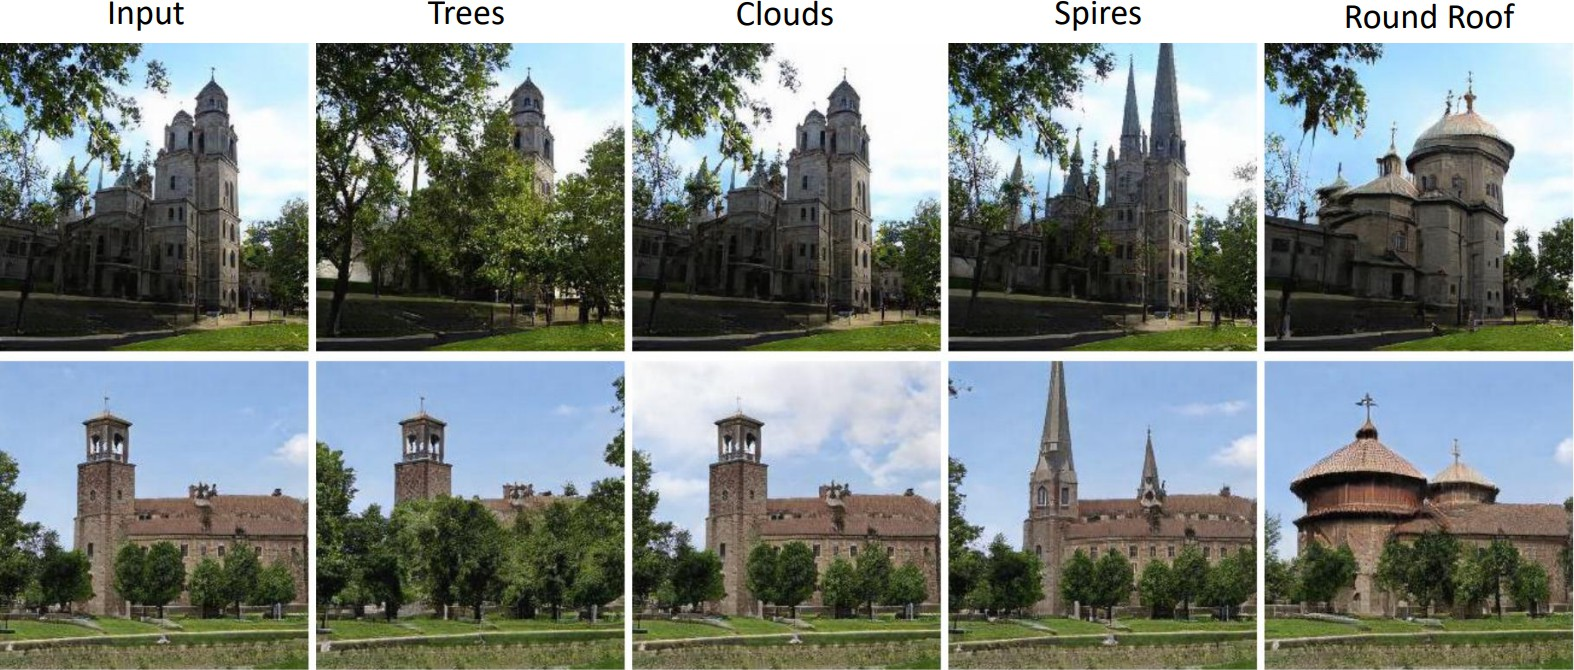
\includegraphics[width=1\textwidth,height=0.9\textheight,keepaspectratio]{images/video/slide_67_1_img.jpg}
    \end{figure}
\end{frame}